\documentclass{deliverablereport}

\deliverable{UI}{ipython-kernels}
\deliverydate{01/02/2018}
\duedate{31/08/2017 (M24)}
\author{Jeroen Demeyer, Sebastian Gutsche, Nicolas M.~Thiéry}

\begin{document}
\maketitle
\tableofcontents

%%%%%%%%%%%%%%%%%%%%%%%%%%%%%%%%%%%%%%%%%%%%%%%%%%%%%%%%%%%%%%%%%%%%%%%%

\section{Introduction}

The \href{https://jupyter.org}{Jupyter Notebook} is a web application
that enables the creation and sharing of executable documents
containing live code, equations, visualizations and explanatory text.
Thanks to a modular design, Jupyter can be used with any computational
system that provides a so-called
\href{https://jupyter.readthedocs.io/en/latest/projects/kernels.html}{\emph{Jupyter kernel}}
to communicate with the notebook.

The Jupyter ecosystem is very large and active: it is being used as a
front-end for scientific research on a daily basis by millions of
scientists around the world, for research, teaching (see
Section~\ref{teaching}) and engineering. The technology goes beyond
the notebook interface, especially with JupyterLab, a recently
released complete refactoring of the Jupyter code base as a flexible
library from which one can build a variety of web-applications,
including live documentation.

\ODK therefore promotes Jupyter as user interface of choice:
it is particularly suitable for building modular web based Virtual Research Environments.

This deliverable is a follow-up to
\delivref{UI}{ipython-kernels-basic}, which dealt with a first basic
version of Jupyter kernels for \ODK's components. We have improved
Jupyter kernels for GAP, PARI/GP, SageMath, and Singular, and made
major contributions to the development of the C++ kernel xeus-cling.
All of them now support syntax highlighting, TAB-completion,
interactive help, and graphics. Some of them also support interactive
widgets.
In addition, we have developed a Jupyter kernel for the MMT system -- the
foundation of knowledge management in OpenDreamKit; this part of the
work is reported on separately in deliverable
\longdelivref{UI}{jupyter-import}.

The components that have been integrated into Jupyter are of very
diverse nature. In particular C++ and MMT are not primarily designed
for Read-Eval-Print Loop user interaction, and we had not foreseen the
feasibility and potential impact of integrating them into Jupyter. Yet
this diversity could be tackled by using a variety of approaches. This
showcases the versatility of the Jupyter technology and its adequation
for building modular Virtual Research Environment.

%%%%%%%%%%%%%%%%%%%%%%%%%%%%%%%%%%%%%%%%%%%%%%%%%%%%%%%%%%%%%%%%%%%%%%%%

\section{Impact}

The implementation of the Jupyter kernels we report on provides all
the computational systems in \ODK with a user-friendly, modern, and
uniform user interface. It further helps users organize, document,
test, share, and publish their work, which supports open science and
reproducibility.

This is a major step for some of the systems that only had a
traditional command-line interface. For the others, it was the
occasion to finally outsource the development of their user
interfaces, which had been a recurrent time sink. For example,
SageMath is dropping the development of its old notebook system
SageNB, refocusing this energy on core business features.

The availability of a Jupyter kernel for C++ extends this to the
interactive use of lower-level computation libraries, within \ODK
(LinBox, MPIR), or beyond (libsemigroups, ...). Contributing to this
kernel was the occasion of interactions and cross-fertilizations with
large scale projects sharing similar needs like CERN's Root.

\subsection{Teaching}\label{teaching}

\begin{figure}\label{AIMS}
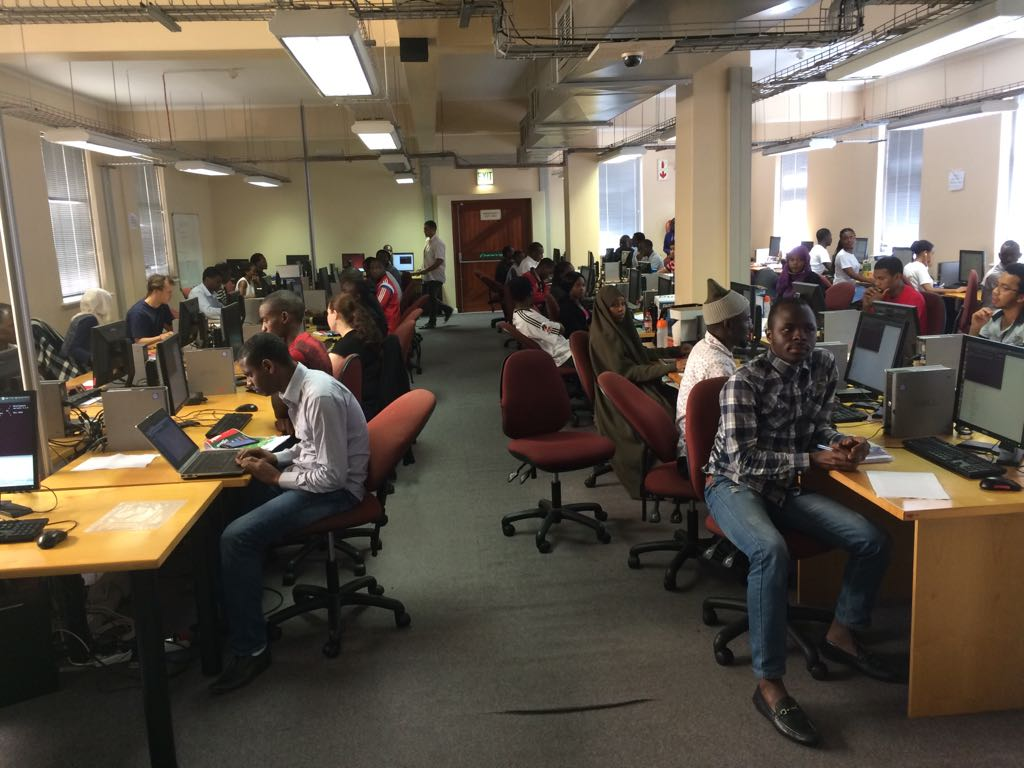
\includegraphics[width=100mm]{IMG-20180124-WA0000.jpg}
\caption{Students at AIMS using the Singular Jupyter interface}
\end{figure}

We showcase here a few of the many uses in teaching of the Jupyter
kernels we contributed to:
\begin{itemize}
\item Since 2017, Jupyter is used at Université Paris Sud for teaching C++ to over 300 students.
This was initiated in particular by \ODK participants Loïc Gouarin, Viviane Pons, and Nicolas M.\ Thiéry.
The mix of narrative documents and interactive programming fostered active participation from the students
while our web-based deployment made it easier for them to work from home.
The course material is available from \url{http://Nicolas.Thiery.name/Enseignement/Info111}.

\item In early spring 2017, Prof.~Dr.~W.~Decker and Prof.~Dr.~G.~Pfister gave a
three-week course on computational algebraic geometry at the
African Institute for Mathematical sciences (Cape Town, South Africa)
with lectures and computer lab sessions.
The course was attended by about 50 students from all over Africa.
In the lab sessions, the students learned how to experiment with the computer algebra system Singular.
It proved extremely valuable that the students could run Singular in the Jupyter notebook.

\item The GAP Jupyter kernel was used by Pedro Garcia-Sanchez to teach
  a master course in mathematical software at the University of
  Granada. See
  \url{https://github.com/pedritomelenas/Software-Matematicas-GAP}.
  Pedro has taken on the technology, and is now involved in the
  development of interactive visualization widgets for discrete maths
  (package francy; see below) in particular for use in other courses.
\end{itemize}

\subsection{Publishing on binder}

Binder (\url{mybinder.org}) is a free web service run by the Jupyter community.
Authors can publish their notebooks there (annotated with a description of their computing environment),
enabling anyone to open and run them from anywhere.
Thanks to our contributions, Binder now support C++, GAP, PARI,
SageMath, or Singular notebooks and has been used for the following
applications:

\begin{itemize}
\item Dissemination: one-click live demos of software packages.
\item Reproducibility: publishing log books documenting the computations underlying a research paper.
\item Live documents: publishing talk slides, course notes, documentation,
      embedding code cells that the reader can modify and execute.
\item Compute service: this is used for example by live documents (see below).
\end{itemize}

\subsection{Live documents with ThebeLab}

\begin{figure}[h]\label{thebelab}
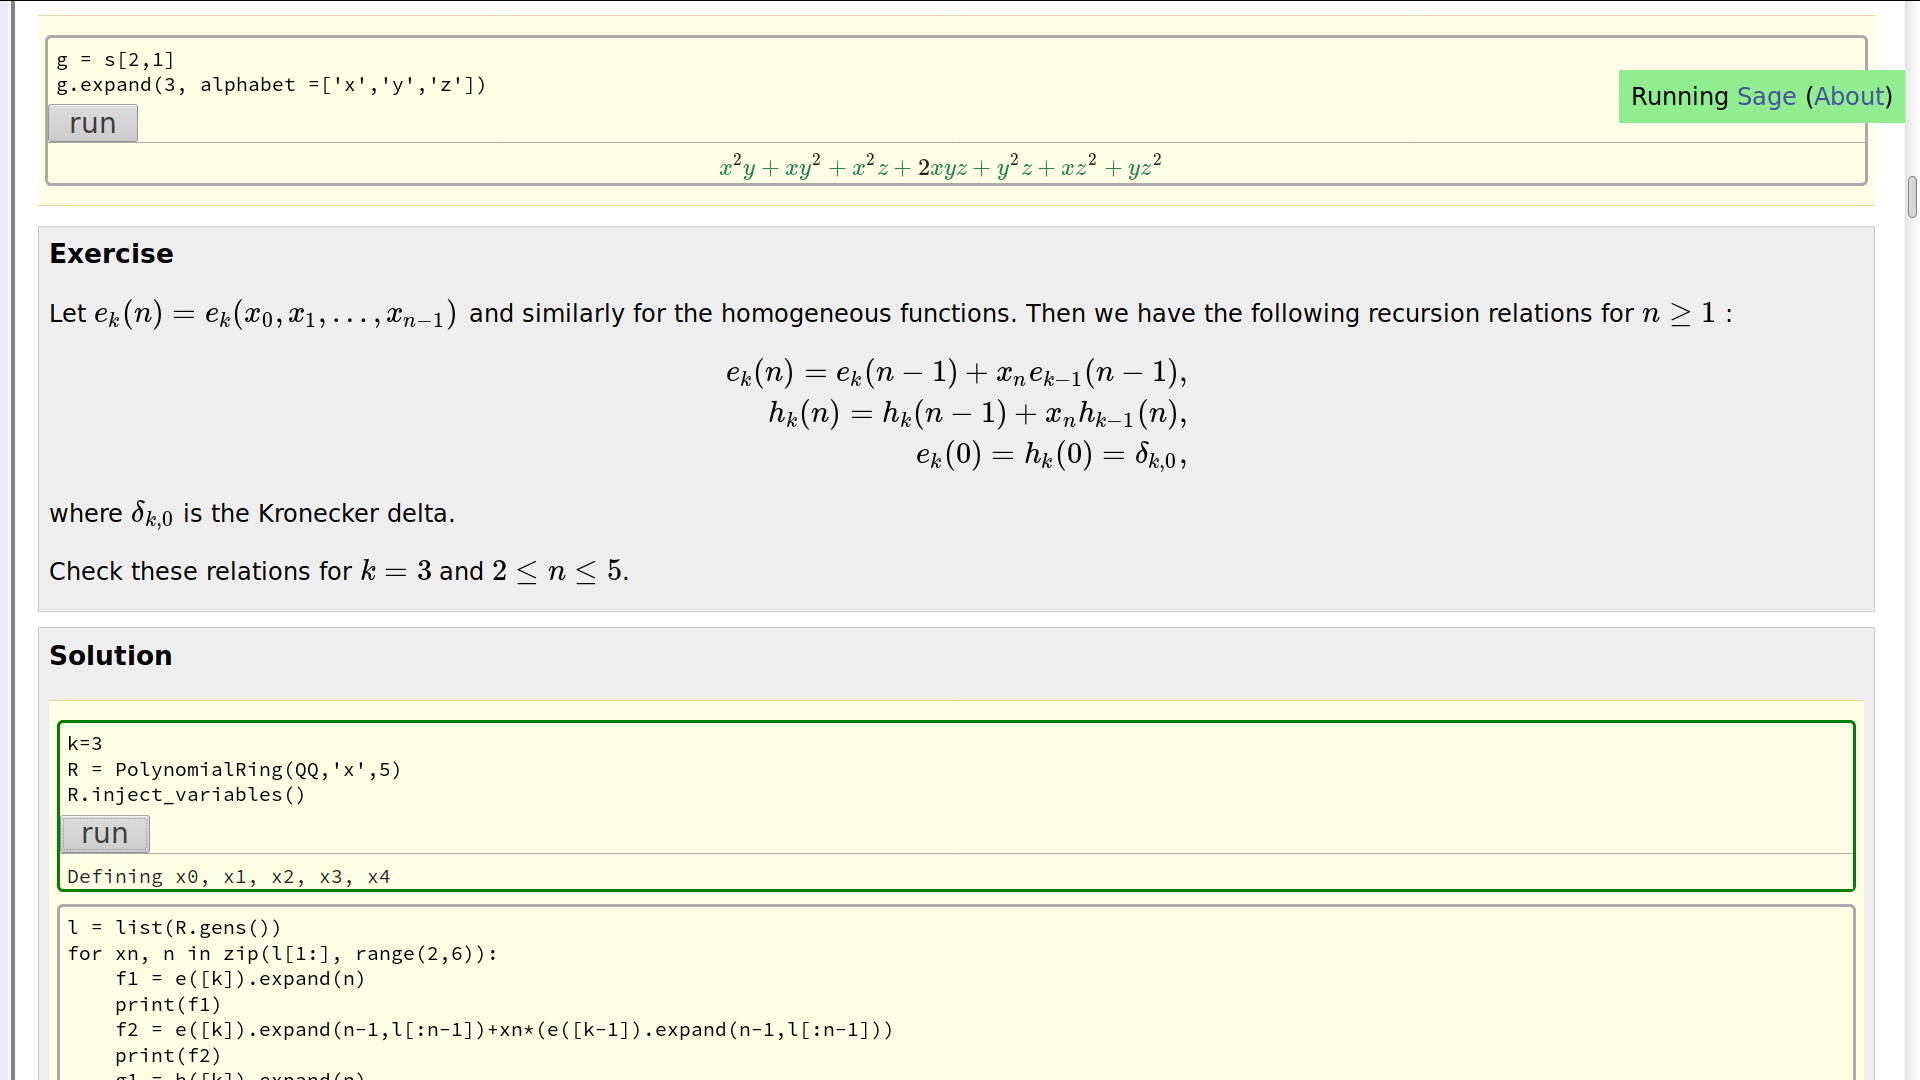
\includegraphics[width=100mm]{thebelab.png}
\caption{SageMath HTML documentation with live code cells thanks to ThebeLab}
\end{figure}

ThebeLab is a JavaScript library for enriching static HTML pages with live code cells
that can be executed and changed by the reader.
Under the hood, the computations can be configured to either run on a free Jupyter hosting service
such as \url{mybinder.org}, or on a custom installation of JupyterHub. Like Jupyter, ThebeLab
is language agnostic, and can now be used with GAP, PARI, SageMath Singular, \ldots

This was originally developed under the name Thebe by O'Reilly Media
for enriching their online books, by forking the Jupyter code base.
At \ODK's workshop on live structured documents in Oslo, Norway in autumn 2017, ThebeLab was
reimplemented by Benjamin Ragan Kelley as a thin layer on top of JupyterLab, with additional
features implemented collaboratively by other participants.

Here are some applications:
\begin{description}
\item[Live documentation for GAP] The GAP system and its packages are documented
inside comments embedded in the code, in the so called AutoDoc format.
This is similar in principle to Javadoc.
The documentation can then be extracted and exported as PDF or HTML.
Thanks to ThebeLab, Binder, and GAP's Jupyter kernel, the HTML documentation can be made live,
letting the user experiment with the provided examples.
Unlike previous implementations, this requires no server-side support, nor changes in the HTML.
The pages can thus be served from anywhere, including e.g. Github Pages.

\item[Live documentation for SageMath] Similarly to the above, SageMath's Sphinx-based documentation system
  can be configured to produce live HTML documentation;
  see figure~\ref{thebelab} for an example.
This is already used by some SageMath packages like
\href{http://more-sagemath-tutorials.readthedocs.io/}{More SageMath Tutorials}
and will soon be used as well by the \Sage's documentation itself.

\item[Live documentation for Singular] It is now possible to convert pages of the Singular
HTML manual into active pages.

\end{description}

%%%%%%%%%%%%%%%%%%%%%%%%%%%%%%%%%%%%%%%%%%%%%%%%%%%%%%%%%%%%%%%%%%%%%%%%

\section{Implementation}

The Jupyter kernels reported on in this report are implemented in a variety of ways, which shows how flexible
the Jupyter protocol is to adapt to various use cases. We now explain some technical details for each of the kernels.

\subsection{GAP}

In the first version we reported on in
\delivref{UI}{ipython-kernel-sage}, the GAP kernel was implemented as
a wrapper kernel. In this use case, this approach proved not flexible
enough for more advanced features. It has thus been reimplemented as a
native kernel, and uses ZeroMQ and GAP's own JSON parser for input and
output, which means the largest part of the protocol is implemented in
plain GAP. In addition, it's now distributed as a standard package of
the GAP distribution. Both versions were implemented in GAP by Markus
Pfeiffer under \ODK funding.

The GAP kernel supports code inspection and completion, as well as
rich output: it is possible to produce any kind of rich output (2D or
3D pictures, latex formulas, widgets, ...) directly from GAP by
returning the appropriate MIME-Types in GAP records.

This is exploited by the GAP package francy
(\url{https://github.com/mcmartins/francy}) by Manuel Martins (with
mentoring from Markus). This package is developed as a Jupyter-based
replacement of the old graphical GAP output in XGAP, and will provide
nice tools to interactively inspect discrete mathematical structures
such as subgroup lattices or conjugacy classes.

\subsection{PARI/GP}

Jeroen Demeyer has implemented a Jupyter kernel for the number-theory package PARI/GP.
The kernel is a wrapper kernel:
it is based on ipykernel, the implementation from IPython of the Jupyter protocol.
Thanks to this, it takes only a small amount of code to write a basic kernel.

It is implemented using the Cython programming language,
which allows for seamless combination of Python code with C code:
Python is used for the interface with the IPython kernel and C is used to execute PARI/GP code
using the PARI library.

Hi-resolution plotting is supported through SVG images: this required significant changes to the PARI/GP
plotting architecture, which previously only worked on the GP command line.

\subsection{Singular}

The Singular kernel is built out of two Python packages: PySingular and jupyter\_kernel\_singular.
Both of these packages are written by Sebastian Gutsche, a regular
\ODK collaborator.

PySingular provides a Python wrapper for Singular's C functions.
It is able to parse Singular code and return either the
output or the resulting error, and to invoke Singular's code completions.
PySingular is written in pure C, using the Python/C API.
To get the full features of Singular, several adjustments in Singular had to be made,
e.g., making Singular's error output available in LibSingular and providing a non-interactive help viewer.

jupyter\_kernel\_singular is a wrapper kernel, based on PySingular's interface to Singular and ipykernel.
It supports all features of the IPython class, such as code inspection, code completion, and completeness check.
Furthermore, it can display pictures of algebraic surfaces
created via the external program surf, which is Singular's main backend for visualisation.

\subsection{SageMath}

Since \Sage is written in Python, its kernel is implemented
on top of the IPython kernel which is very rich by itself.
Additional work included:
\begin{itemize}
\item Configuration of the documentation.
\item Rich output handling (LaTeX with mathjax, plots, ...).
\item Improvements to Jupyter's widgets and interact functionality to be as feature rich as in the old \Sage Notebook.
\end{itemize}
The last item was implemented by Jeroen Demeyer under \ODK funding as part of \longdelivref{UI}{ipython-kernel-sage}.
Most of the rest was implemented by the \Sage community.

\subsection{C++: xeus-cling}

\texttt{xeus-cling} is based on xeus, a native C++ implementation of
the Jupyter protocol, and Cling, a C++ interpreter based on the C++
compiler Clang and compiler suite LLVM. \ODK contributed man power
with Loïc Gouarin being one of the main developers. Also Nicolas M.
Thiéry was an early adopter (beta-test, bug reports, feature
suggestions, promotion).

\subsection{MMT}

As part of \longdelivref{UI}{jupyter-import}, Florian Rabe et al.
implemented a kernel for
\href{https://uniformal.github.io/}{MMT}, a framework for
(mathematical) knowledge management which is the workhorse behind
\url{mathhub.info} and OpenDreamKit's Math-in-the-Middle approach.
MMT's specialty is the representation of arbitrary declarative
languages such as logics, type theories, set theories, etc, and
implements complex algorithms generically for any language in the
framework.

MMT's Jupyter kernel is based on the feature-rich Python kernel
(widgets, ...), using the Py4J Python-Java bridge to interact easily
with MMT (which is implemented in the Java-compatible Scala language). See
\delivref{UI}{jupyter-import} for screenshots and implementation
details. The biggest part of the work was to design the desirable interactive
interaction with MMT as its nature is rather different from
conventional computational systems. The shear fact that it was
possible illustrates well the versatility of the Jupyter architecture.

%%%%%%%%%%%%%%%%%%%%%%%%%%%%%%%%%%%%%%%%%%%%%%%%%%%%%%%%%%%%%%%%%%%%%%%%
\clearpage
\appendix
\section{Screenshots}
\newcommand{\screenshot}[2]{
\begin{figure}[ht]
  \includegraphics[width=\textwidth,trim={0 0 0 1px},clip]{#1}
  \caption{#2}
\end{figure}}

\screenshot{pari.png}{PARI/GP Jupyter kernel}
\screenshot{sage.png}{SageMath Jupyter kernel}
\screenshot{singular_new.png}{Singular Jupyter kernel}
\clearpage
\screenshot{gap.png}{GAP Jupyter kernel with package francy}
\clearpage
\screenshot{cling-teaching.png}{A C++ exercise sheet using the Jupyter kernel xeus-cling}
\end{document}
